\chapter{Lead us not into temptation (Vibrate High)}
\vspace{0.6cm}
\begin{center}
\nopagebreak
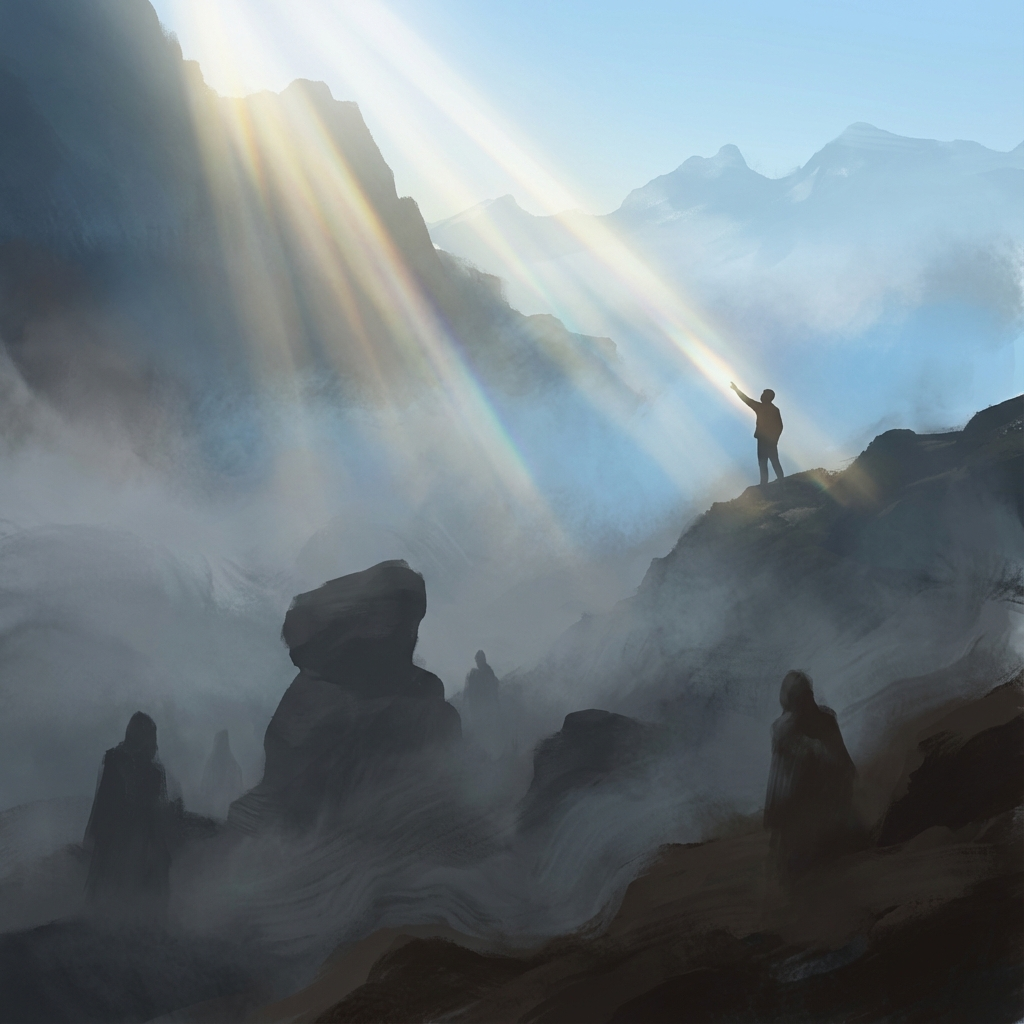
\includegraphics[width=0.75\textwidth,cfbox=gray!60 0.6pt 4pt]{fog_light.png}\\
\vspace{4pt}
{\small\itshape Vibrating high: rising above dense emotions.}
\end{center}

\vspace{0.6cm}
We were back in Colmenarejo, walking along a path surrounded by rockroses. The smell of the countryside was intense.
—Temptation —Jesus said, plucking a sprig of rosemary—. What do you think it is?


—Chocolate? Easy money?


—Those are distractions. The true temptation is to lower your vibration. It is the temptation to fall into fear, into anger, into despair.


He stopped and looked into my eyes.
—``Lead us not into temptation'' means: ``Help me stay vibrating high''. Because when you vibrate high, you are in your power. When you fall, you lose your connection.


—But sometimes getting angry is inevitable.


—It is inevitable to feel the emotion, yes. But it is optional to stay and live in it. The temptation is to wallow in drama. It's calling your friend to tell her for the tenth time how badly your boss treated you, just to feel that rage again. That is falling into temptation. It is choosing suffering because it makes you feel important, a victim.


—And how is it avoided?


—With awareness. When you feel that you are going to fall, that you are going to start complaining or criticizing, stop. Breathe. Remember who you are. Remember that you are light. And choose again. Choose gratitude. Choose hope. Choose love. That is vibrating high. And there, temptation has no strength.